\chapter{Experimental Setup}
\label{ch:setup}

\section{Datasets and Preprocessing}
\label{sec:data}

\subsection{Network topologies}

Five topologies from the Internet Topology Zoo~\cite{knight2011zoo} were used, spanning a twenty-fold range in size (Table~\ref{tab:topologies}). Each GML file is parsed with NetworkX~\cite{hagberg2008networkx}. Self-loops are removed and parallel edges are merged. Node coordinates come from the GML attributes or, for OS3E, from a table of city coordinates. Shortest-path delays and controller hosts are then computed as in Section~\ref{sec:system-model}. Because the number of switches $N$ fixes the state and action dimensions, a separate agent is trained for each topology.

\begin{table}[htbp]
\centering
\caption{Topologies, selected controller hosts and resulting problem dimensions.}
\label{tab:topologies}
\small
\fitwidth{\begin{tabular}{@{}lrrP{4.6cm}rrr@{}}
\toprule
\textbf{Topology} & \textbf{$N$} & \textbf{Links} & \textbf{Controller hosts ($c_0$ first)} & \textbf{max $D$ (ms)} & \textbf{State (cur./pred.)} & \textbf{$|\mathcal{A}|$}\\
\midrule
Gridnet    & 9   & 20  & San Francisco, Newark, Atlanta, Dallas, Houston, Los Angeles & 21.50 & 21 / 36 & 20\\
BellCanada & 48  & 64  & Edmonton, Seattle, Vancouver, Calgary, Quebec City, Montreal & 38.06 & 60 / 114 & 59\\
OS3E       & 34  & 36  & Stockholm, Paris, Hamburg, Vienna, London, Brussels & 18.14 & 46 / 86 & 45\\
Interoute  & 110 & 146 & Timisoara, London, Paris, Marseille, Sofia, Strasbourg & 19.47 & 122 / 238 & 121\\
Cogentco   & 197 & 243 & Paris, London, Cleveland, Washington, Frankfurt, Bratislava & 59.47 & 209 / 412 & 208\\
\bottomrule
\end{tabular}}
\end{table}

\subsection{Synthetic temporal traffic}

No public dataset provides switch-level controller load for these five topologies, so a reproducible generator was written in NumPy. For each topology it produces 20,000 normalised switch-load rows, with one row per decision interval and 60 rows per simulated hour. The load of switch $i$ at step $t$ is the product of several factors:
\begin{itemize}[leftmargin=*]
  \item a day/night profile (0.20 at night up to 0.92 at midday, scaled per topology);
  \item a slow daily wave and a per-switch phase-shifted short wave;
  \item random bursts lasting 12--48 steps;
  \item periodic \emph{cool-down} windows that create parking opportunities;
  \item persistent hotspot switches and periodic rebalancing pressure on a random 18\% of switches;
  \item a per-switch bias and Gaussian noise.
\end{itemize}
The result is smoothed by an exponential memory term (0.82--0.88) and clipped to $[0,1]$. Larger topologies are given more frequent and stronger bursts, so that difficulty grows with size. The mean switch load ranges from 0.59 (Gridnet) to 0.76 (Cogentco). Each trace is split \emph{chronologically}, without shuffling, into 70\% training (14,000 rows), 15\% validation (3,000) and 15\% test (3,000). Figure~\ref{fig:traffic}(a) shows a segment of the OS3E trace. The generator is a controlled stress test for threshold-crossing behaviour; it is not a model of any specific operator's traffic.

\begin{figure}[htbp]
  \centering
  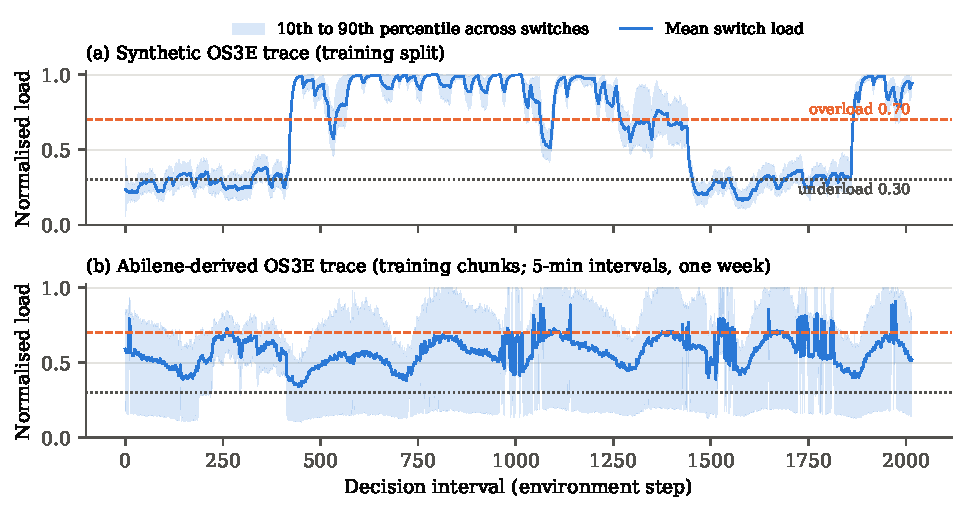
\includegraphics[width=\textwidth]{traffic_traces}
  \caption{Mean and 10th--90th percentile switch load over the first 2,016 steps of (a) the synthetic OS3E training split and (b) the Abilene-derived OS3E training split. Dashed and dotted lines mark the overload and underload thresholds.}
  \label{fig:traffic}
\end{figure}

\subsection{Abilene-derived real-traffic case study}
\label{sec:abilene}

To test the framework on measured traffic dynamics, the Abilene/Internet2 traffic-matrix archive~\cite{zhang2004abilene,zhang2003tm} was used. It provides $12\times12$ origin--destination (OD) matrices at 5-minute intervals in weekly chunks (\texttt{X01}--\texttt{X24}, 2,016 matrices each, 2004). Preprocessing (SHA-256 of the archive recorded) consists of four steps:
\begin{enumerate}[leftmargin=*]
  \item extract the measured OD component of each matrix and remove the diagonal;
  \item convert it to a 12-node load vector by summing each node's ingress and egress demand;
  \item project the 12 Abilene nodes onto the 34 OS3E switches with a fixed, documented two-source mapping (switch $i$ receives 0.80 of node $i \bmod 12$ and 0.20 of a second node);
  \item normalise each switch by the 99th percentile of the \emph{training} portion only, then clip to $[0,1]$.
\end{enumerate}
The result keeps the temporal structure of real backbone demand. It is \emph{not} measured OS3E traffic, and is referred to throughout as an \emph{Abilene-derived trace mapped to OS3E}.

Two isolated protocols were built from the archive:
\begin{itemize}[leftmargin=*]
  \item \textbf{Zero-shot transfer:} chunks \texttt{X06}--\texttt{X20} (30,240 steps) split 70/15/15. Only the 4,536-step test portion was used, to evaluate synthetic-trained OS3E models without any retraining.
  \item \textbf{Real-data training:} a fresh chunk-level split with training \texttt{X06}--\texttt{X14} (18,144 steps), validation \texttt{X15}--\texttt{X17} (6,048) and final test \texttt{X21}--\texttt{X24} (8,064). Chunks \texttt{X18}--\texttt{X20} were \emph{excluded} because they overlap the zero-shot evaluation window.
\end{itemize}
The real trace is markedly less stressed than the synthetic one. In the training data, 14\% of switch-load values exceed 0.70, against 59\% for synthetic OS3E (mean load 0.44 versus 0.70; Figure~\ref{fig:traffic}(b)).

\section{Implementation Details}
\label{sec:impl}

The framework was implemented in Python 3.10.14. Table~\ref{tab:software} lists the main libraries and Table~\ref{tab:modules} the modules. All training and evaluation ran on a CPU-only laptop (Intel Core~5~120U, 12 logical cores, 16\,GB RAM, Ubuntu 24.04); no GPU was used. Each run writes its checkpoint together with a JSON metadata file recording the state and action dimensions, hyperparameters, seed, traffic file, reward version (\path{normalized_multi_objective_v2}) and action-schema version (\path{stable_controller_slots_v2}). An evaluation refuses to load a checkpoint whose dimensions do not match the environment. Training was logged to TensorBoard, and evaluation results were written as CSV and JSON. A suite of eight unit tests (Appendix~\ref{app:verification}) checks the invariants that earlier bugs had violated, and all eight pass on the final code.

\begin{table}[htbp]
\centering
\caption{Software environment.}
\label{tab:software}
\small
\begin{tabular}{@{}ll@{}}
\toprule
\textbf{Component} & \textbf{Version / role}\\
\midrule
Python & 3.10.14\\
PyTorch~\cite{paszke2019pytorch} & 2.9.1 (CPU execution) -- Rainbow DQN and GRU\\
Gymnasium~\cite{towers2024gymnasium} & 1.2.3 -- environment interface\\
NetworkX~\cite{hagberg2008networkx} & 3.4.2 -- topology parsing, shortest paths, centrality\\
NumPy & 2.2.6 -- traffic generation and preprocessing\\
TensorBoard / Matplotlib & 2.20.0 / 3.10.8 -- logging and figures\\
\bottomrule
\end{tabular}
\end{table}

\begin{table}[htbp]
\centering
\caption{Main implementation modules.}
\label{tab:modules}
\small
\begin{tabularx}{\textwidth}{@{}P{6.4cm}L@{}}
\toprule
\textbf{Module} & \textbf{Responsibility}\\
\midrule
\path{utils/topology_loader.py} & GML parsing, haversine delays, shortest-path matrix, controller hosts\\
\path{experiments/preprocessing/create_synthetic_traffic.py} & Synthetic switch-load generator\\
\path{experiments/preprocessing/split_traffic_temporal.py} & Chronological 70/15/15 split with manifest\\
\path{experiments/preprocessing/prepare_abilene_*.py} & Abilene-to-OS3E projection and splits\\
\path{environments/threshold_proactive_sdn_env.py} & Environment: state, valid actions, feasibility, reward, metrics\\
\path{environments/rainbow_dqn_model.py} & Noisy dueling C51 network, PER, $n$-step buffer, projection, update\\
\path{forecasting/gru_traffic_predictor.py} & GRU network and frozen inference wrapper\\
\path{experiments/train_rainbow_fixed_rewards.py} & RDQN training (current/predictive), checkpoint metadata\\
\path{experiments/train_gru_forecaster.py} & GRU training, early stopping, persistence comparison\\
\path{experiments/evaluate_fair_baselines.py} & Identical-condition evaluation of RDQN and baselines\\
\path{experiments/evaluate_real_traffic_zero_shot.py} & Evaluation on an explicitly supplied real-derived trace\\
\path{tests/test_sdn_core.py} & Regression tests of environment and Rainbow invariants\\
\bottomrule
\end{tabularx}
\end{table}

\section{Experimental Settings}
\label{sec:settings}

\paragraph{Hyperparameters.} Table~\ref{tab:hyper} gives the Rainbow settings. Capacity scales with topology size, and the values were fixed before the final experiments. Common settings are $\gamma=0.99$, 51 atoms on $[-10,10]$, Adam, $\varepsilon$ decaying from 0.10 to 0.01 (time constant $0.6T$), one update per four steps after 1,000 warm-up steps, a target copy every 1,000 steps and 1,000-step training episodes.

\begin{table}[htbp]
\centering
\caption{Topology-dependent Rainbow DQN hyperparameters and recorded CPU training time.}
\label{tab:hyper}
\small
\fitwidth{\begin{tabular}{@{}lccccccc@{}}
\toprule
\textbf{Topology} & \textbf{Hidden $H$} & \textbf{LR} & \textbf{$n$} & \textbf{Batch} & \textbf{Buffer} & \textbf{Steps} & \textbf{Time (min)}\\
\midrule
Gridnet    & 128 & $2\times10^{-4}$ & 3 & 64  & 30k  & 80k  & 31.4 / 44.7\\
BellCanada & 256 & $1\times10^{-4}$ & 3 & 128 & 50k  & 80k  & 56.4 / 77.9\\
OS3E       & 256 & $1\times10^{-4}$ & 3 & 128 & 50k  & 80k  & 48.1 / 69.8\\
Interoute  & 512 & $5\times10^{-5}$ & 5 & 256 & 100k & 80k  & 143.0 / --\\
Cogentco   & 512 & $5\times10^{-5}$ & 5 & 256 & 100k & 80k, 120k & 222.8, 313.8 / --\\
\bottomrule
\end{tabular}}
\par\smallskip\footnotesize Time is current / predictive mode for the synthetic models. Real-data OS3E models took about 40\,min (current) and 50--52\,min (predictive) per seed.
\end{table}

\paragraph{Evaluation protocol.} A single evaluator runs every policy with the same topology, trace split, thresholds, reward, seed and evaluation windows. Each evaluation uses six episodes of 500 steps (3,000 decisions per policy), with start indices spread evenly across the split, $\text{start}_e=\lfloor e(L-500)/5\rfloor$ for $e=0,\dots,5$. Windows never wrap around the end of the split. The learned policy acts greedily over valid actions with noise disabled, and no learning occurs during evaluation. Validation runs use evaluation seed 1042 and final tests use seed 2042; models are trained with seed 42 unless stated otherwise.

\paragraph{Model selection and test discipline.} Figure~\ref{fig:protocol} shows the workflow. All tuning decisions were made on validation data:
\begin{itemize}[leftmargin=*]
  \item predictive RDQN was trained only for the topologies where the GRU beat persistence;
  \item a horizon-3 GRU was tried for Gridnet and BellCanada;
  \item the observation mode was chosen per topology;
  \item Cogentco was retrained with 120k steps after its 80k model under-performed on validation.
\end{itemize}
The configurations were then frozen and each test split was evaluated once. The validation run of the 120k Cogentco model was not recorded before its test evaluation. That result therefore lacks a validation confirmation, which is noted as a limitation. Only one Cogentco checkpoint was ever evaluated on the test split, so no selection among test results took place. For the real-data study, the seed-42 configuration was frozen after validation and then replicated unchanged with seeds 43 and 44, retraining both the GRU and the RDQN.

\begin{figure}[htbp]
  \centering
  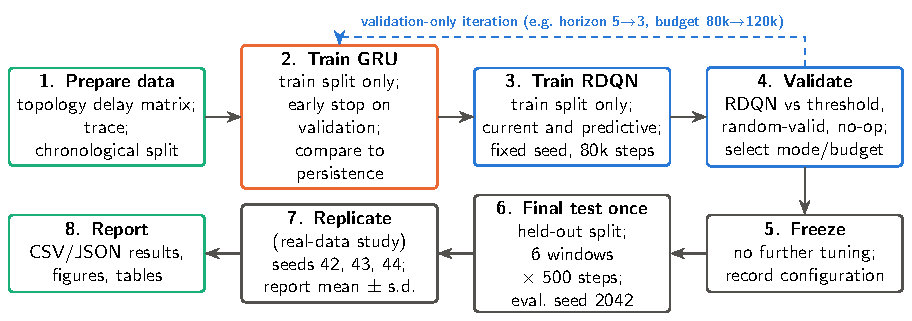
\includegraphics[width=\textwidth]{protocol}
  \caption{Experimental workflow. Iteration (dashed) used validation data only; each test split was used once, after freezing.}
  \label{fig:protocol}
\end{figure}

\begin{table}[htbp]
\centering
\caption{Summary of the three experimental protocols.}
\label{tab:protocols}
\small
\begin{tabularx}{\textwidth}{@{}p{3.0cm}LLL@{}}
\toprule
 & \textbf{Synthetic (E1)} & \textbf{Zero-shot real (E2)} & \textbf{Real-data-trained (E3)}\\
\midrule
Topologies & All five & OS3E & OS3E\\
Training traffic & Synthetic train split & Synthetic (no retraining) & Abilene \texttt{X06}--\texttt{X14}\\
Selection traffic & Synthetic validation split & -- & Abilene \texttt{X15}--\texttt{X17}\\
Test traffic & Synthetic test split & Abilene \texttt{X06}--\texttt{X20} test 15\% & Abilene \texttt{X21}--\texttt{X24}\\
Modes & Selected per topology & Current and predictive & Current and predictive\\
Training seeds & 42 & 42 & 42, 43, 44\\
Evaluation & $6\times500$, seed 2042 & $6\times500$, seed 2042 & $6\times500$, seed 2042\\
\bottomrule
\end{tabularx}
\end{table}

\section{Evaluation Criteria and Performance Metrics}
\label{sec:metrics}

Metrics are recorded at every evaluation step and aggregated as in Table~\ref{tab:metrics}. Cumulative reward is the primary criterion because it is the objective the agent optimises and it combines all three costs. Individual metrics are reported alongside it so that trade-offs are visible: a policy can improve the reward while losing on one metric. Rewards are comparable only within one protocol and observation mode, because the traffic and valid action sets differ between them.

\begin{table}[htbp]
\centering
\caption{Performance metrics.}
\label{tab:metrics}
\small
\begin{tabularx}{\textwidth}{@{}p{3.6cm}L@{}}
\toprule
\textbf{Metric} & \textbf{Definition (direction)}\\
\midrule
Cumulative reward & Sum of $r_t$ over a 500-step episode, averaged over six episodes (higher is better)\\
Average latency & Mean over switches of $D_{i,m(i)}$, averaged over steps (ms, lower)\\
Worst-case latency & Maximum assigned switch--controller delay in an episode, averaged over episodes (ms, lower)\\
Energy & Mean controller-state energy $E_t$ (W, lower)\\
Load index & Standard deviation of the number of switches per active controller (lower is more even)\\
Traffic balance & Coefficient of variation of active-controller loads (lower)\\
Overload / underload \% & Share of steps with at least one controller above 0.70 / below 0.30 before acting (lower)\\
Action counts, failures & Successful park, evoke and migrate actions per episode; failed actions\\
Forecast MAE & $\frac1N\lVert\hat{\mathbf{x}}_{t+h}-\mathbf{x}_{t+h}\rVert_1$ during evaluation (predictive mode)\\
Forecast-only actions & Successful evoke/migrate actions taken when overload was forecast but not current\\
GRU quality & Validation MAE, RMSE and overload F1 versus the persistence forecast\\
\bottomrule
\end{tabularx}
\end{table}
